\documentclass[windows,csize4]{BHCexam}
%\documentclass[windows,csize4,answers]{BHCexam}

\usepackage{multicol} % 分栏
\usepackage{polynom} % 多项式除法
\pagestyle{fancy}
\fancyfoot[C]{\kaishu \small 第 \thepage 页 共 \pageref{lastpage} 页}
%\fancyhead[L]{\includegraphics[width=2cm]{qrcode.png}}
\title{因式分解 - 对称式和轮换式}
%\subtitle{数学文科试卷}
%\notice{满分150分, 120分钟完成, \\	允许使用计算器,答案一律写在答题纸上.}
%\author{Gavin Chen}
%\date{\today}
\usepackage{enumerate} % 编号
\usepackage{cases}
\usepackage{subfigure}
\usepackage{graphicx}

\begin{document}

\maketitle

\begin{groups}
    \group{前言}{}
    物理学是一门怎样的学科。
    \begin{itemize}
        \item 物理——万物之理。
        \item 实践是一切知识的试金石;实验是科学“真理”的唯一鉴定者。
        \item 物理学中的分工:理论物理学家想象、推演和猜测新的定律;实验物理学家进行实验、想象、推演和猜测。
    \end{itemize}
    
    \group{长度的测量}{}
    关于测量,眼见不一定为实,所以需要测量。
    图 \ref{fig:fig_1_1}中$AB$,$CD$哪个线段更长?
    \begin{figure}[htb]
        \centering
        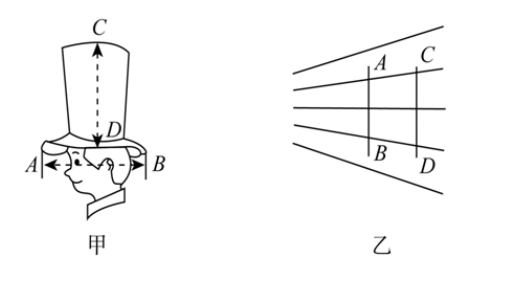
\includegraphics [scale=0.75,trim=0 0 0 0]{./image/fig_1_1.PNG}
        \caption{$AB$,$CD$哪个线段更长} 
        \label{fig:fig_1_1}
    \end{figure}

    图 \ref{fig:fig_1_2}中$AB$,$CD$是否平行?$EFGH$是否是正方形?
    \begin{figure}[htb]
        \centering
        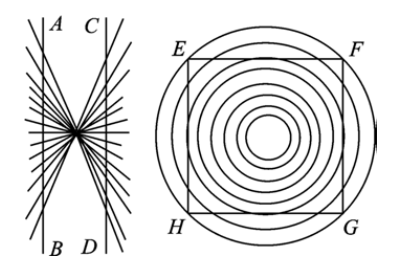
\includegraphics [scale=0.75,trim=0 0 0 0]{./image/fig_1_2.PNG}
        \caption{$AB$,$CD$是否平行?$EFGH$是否是正方形} 
        \label{fig:fig_1_2}
    \end{figure}

    测量及其单位:将待测量与标准量进行比较。
    \begin{itemize}
        \item 测量需要标准,这个用来比较的标准量叫做单位。
        \item 国际单位制,国际计量组织指定的一套国际统一的单位。
        \item 国际单位制中,长度的单位是米, 符号$m$,其他还有千米($km$),分米($dm$),厘米($cm$),毫米($mm$),
        微米($\mu m$),纳米($nm$)等。
    \end{itemize}

    常见物体的长度:
    \begin{itemize}
        \item  原子-埃($10^{-10}$),纳米-分子,微米-体细胞,毫米-笔芯
        \item 地球周长:4万千米,太阳到地球:1.5亿千米(一个天文单位),比邻星 4.2光年,银河系:10万光年
    \end{itemize}


    常见长度测量工具:刻度尺,游标卡尺,千分尺(螺旋测微器)
    \begin{figure}[htb]
        \centering
        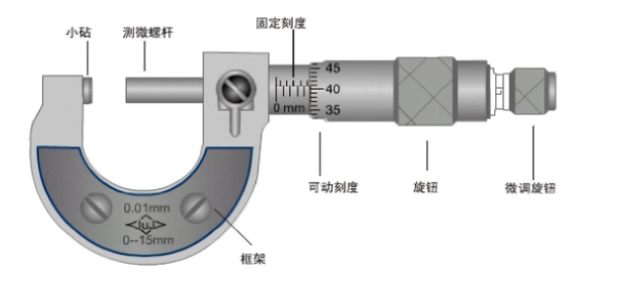
\includegraphics [scale=0.25,trim=0 0 0 0]{./image/fig_1_3.PNG}
        \caption{千分尺} 
        \label{fig:fig_1_3}
    \end{figure}
    \begin{figure}[htb]
        \centering
        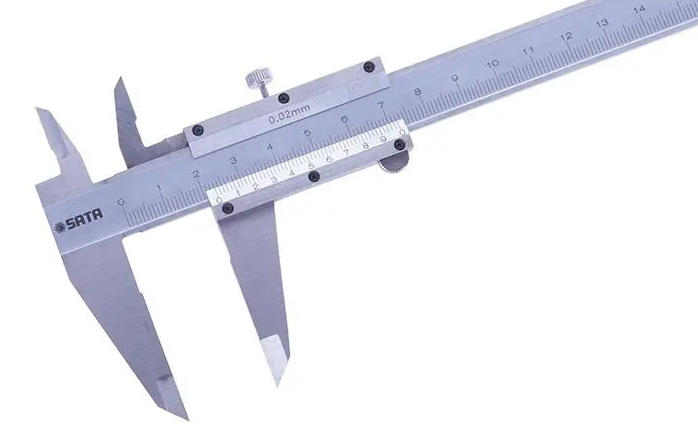
\includegraphics [scale=0.25,trim=0 0 0 0]{./image/fig_1_4.PNG}
        \caption{游标卡尺} 
        \label{fig:fig_1_4}
    \end{figure}

    关于刻度尺的量程和最小刻度,如图\ref{fig:fig_1_5}
    \begin{figure}[htb]
        \centering
        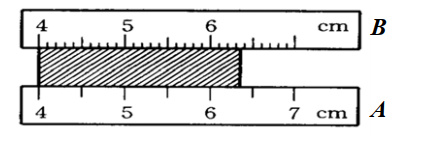
\includegraphics [scale=0.75,trim=0 0 0 0]{./image/fig_1_5.PNG}
        \caption{A、B测量结果有何不同?} 
        \label{fig:fig_1_5}
    \end{figure}

    注意:长度需要估读最小分度的下一位。

\group{特殊的测量方法}{}
\begin{itemize}
    \item 组合平移
    \item 化曲为直
    \item 化曲为直(滚动)
    \item 积累法
\end{itemize}
常见特殊测量方法如图\ref{fig:fig_1_7_10}所示。
\begin{figure}
    \centering
    \begin{minipage}{5cm}
        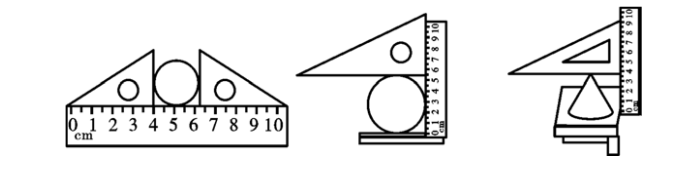
\includegraphics[width=5cm]{./image/fig_1_7.PNG}
    \end{minipage}
    \begin{minipage}{5cm}
        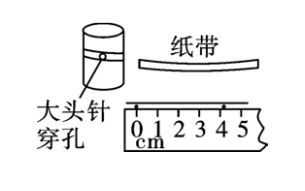
\includegraphics[width=5cm]{./image/fig_1_8.PNG}
    \end{minipage}


    \begin{minipage}{5cm}
        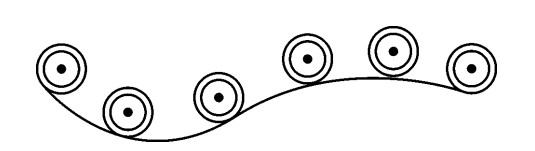
\includegraphics[width=5cm]{./image/fig_1_9.PNG}
    \end{minipage}
    \begin{minipage}{5cm}
        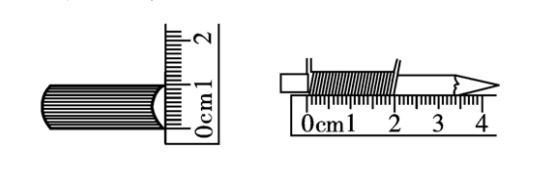
\includegraphics[width=5cm]{./image/fig_1_10.PNG}
    \end{minipage}   
\caption{特殊的测量方法} 
\label{fig:fig_1_7_10}
\end{figure}


\group{误差和错误}{}
误差——真值和测量值之间的差异。
\begin{itemize}
    \item 误差不是错误,测量错误应该要避免。
    \item 误差总是存在,不可避免。
    \item 减小误差的方法:
    \begin{itemize}
        \item 多次测量求平均
        \item 使用更加精密的测量工具
    \end{itemize}

\end{itemize}

\group{面积的测量}{}

面积测量的方法,如图\ref{fig:fig_1_6}
\begin{figure}[htb]
    \centering
    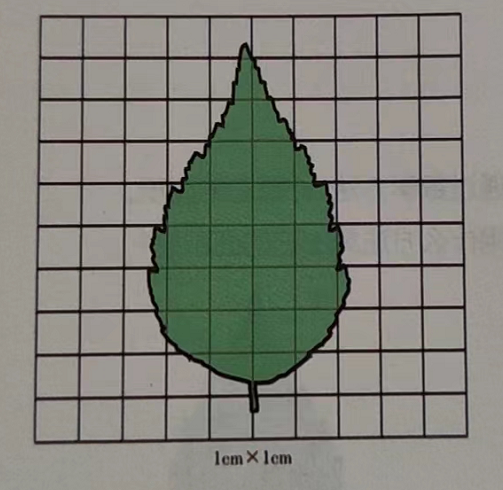
\includegraphics [scale=0.35,trim=0 0 0 0]{./image/fig_1_6.PNG}
    \caption{如何测量面积} 
    \label{fig:fig_1_6}
\end{figure}

补充知识,油膜法测分子直径

\group{质量和体积的测量}{}
质量的单位:千克($kg$),克($g$)等。
体积的单位:立方米($m^3$),升($L$),毫升($mL$)等。

常用测量工具:天平(图\ref{fig:fig_1_11}),电子天平(图\ref{fig:fig_1_11}),量筒等。
\begin{figure}[htb]
    \centering
    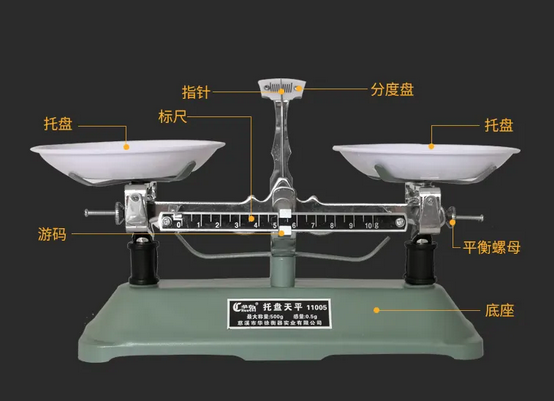
\includegraphics [scale=0.5,trim=0 0 0 0]{./image/fig_1_11.PNG}
    \caption{天平} 
    \label{fig:fig_1_11}
\end{figure}
\begin{figure}[htb]
    \centering
    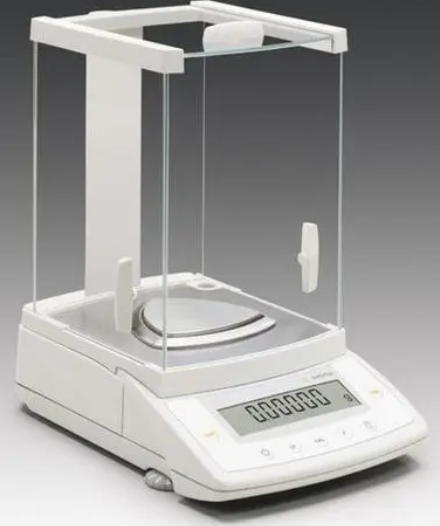
\includegraphics [scale=0.5,trim=0 0 0 0]{./image/fig_1_12.PNG}
    \caption{电子天平} 
    \label{fig:fig_1_12}
\end{figure}

量筒的正确测量方法:

\begin{figure}[htb]
    \centering
    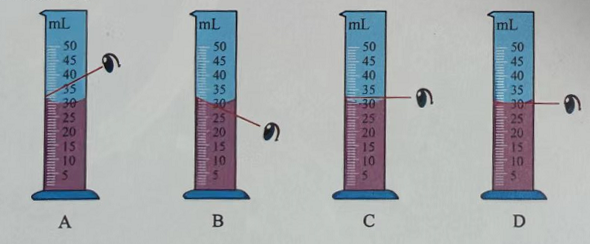
\includegraphics [scale=0.5,trim=0 0 0 0]{./image/fig_1_13.PNG}
    \caption{如何用量筒测量?} 
    \label{fig:fig_1_13}
\end{figure}
想一想:如何测量小石子的体积?

\question[5]甲、乙两同学分别用量筒测量一个小石块的体积。甲同学的做法是在量简里注入适量的水,记下水的体$V_1$,
然后轻轻放入石块,使量简里的水完全浸没石块,记下此时水及石块的体积 $V_2$,计算石块的体积为$V_2-V_1$。
乙同学是先将石块置于量筒中,同时往量筒中注入水,使水全部浸没石块记下总的体积 $V_2$,然后取出石块,记下取出石块后水的体积$V_1$,计算石块的体积为$V_2-V_1$。
\begin{subquestions}
    \subquestion 你做此实验将选择哪种方法?
    \subquestion 如果两同学读数都是正确的,两同学计算出的石块体积可能不相等,比较大的是谁?
\end{subquestions}
\begin{solution}{0.5cm}
    \methodonly
\end{solution}

\group{时间的测量}{}
 时间的单位:秒($s$)
 
 打点计时器, 如图\ref{fig:fig_1_14}所示。一般工作电压$4V-6V$,当频率$f=50Hz$时,它每隔$0.02s$打一个点。
 \begin{figure}[htb]
    \centering
    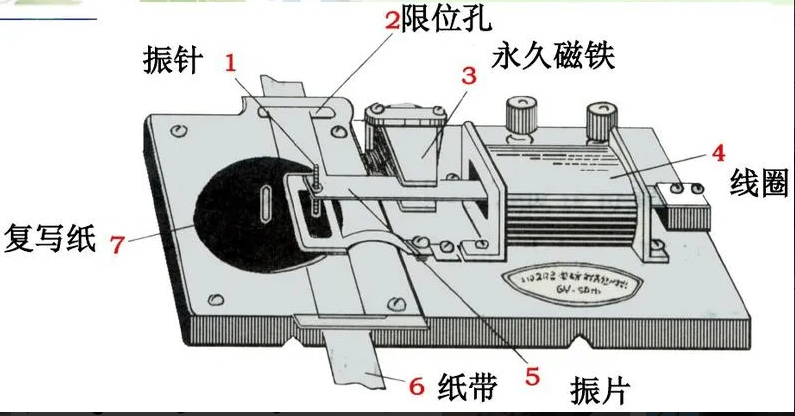
\includegraphics [scale=0.5,trim=0 0 0 0]{./image/fig_1_14.PNG}
    \caption{打点计时器} 
    \label{fig:fig_1_14}
\end{figure}

\question[5] 甲、乙两位同学用打点计时器打出的纸带分别如图\ref{fig:fig_1_15}所示,其中甲同学纸带中从$A$ 点到$H$点经历的时间为
多少秒?通过比较可以知哪位同学拉纸带比较快?
\begin{figure}[htb]
    \centering
    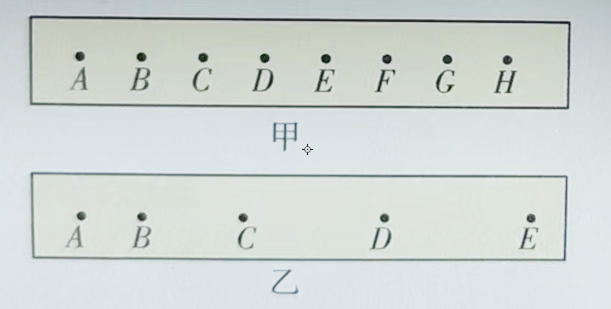
\includegraphics [scale=0.5,trim=0 0 0 0]{./image/fig_1_15.PNG}
    \caption{纸带上的点} 
    \label{fig:fig_1_15}
\end{figure}

单摆。
单摆的模型:悬挂小球的细线质量相对于小球可以忽略,且不可伸缩。线长远大于球的直径,这样的装置叫做单摆。
\begin{itemize}
    \item 单摆是理想化的模型
    \item 摆长和线长不同,摆长是悬点到小球重心的距离。
    \item 研究方法:控制变量法。
\end{itemize}

\begin{itemize}
    \item 角度很小时($<5^o$),具有等时性(伽利略)。
    \item 单摆周期$T=2\pi \sqrt{\frac{L}{g}}$
    \item 同一地点(即$g$不变),周期只与摆长有关。
\end{itemize}

想一想,如果我们要研究单摆,应该如何控制变量? 
\question[5] 小明做了四次实验,记录如表\ref{fig:fig_1_16}所示。
\begin{subquestions}
    \subquestion 分析1,2次实验,可以得到什么结论?
    \subquestion 分析1,3次实验,可以得到什么结论?
\end{subquestions}
\begin{figure}[htb]
    \centering
    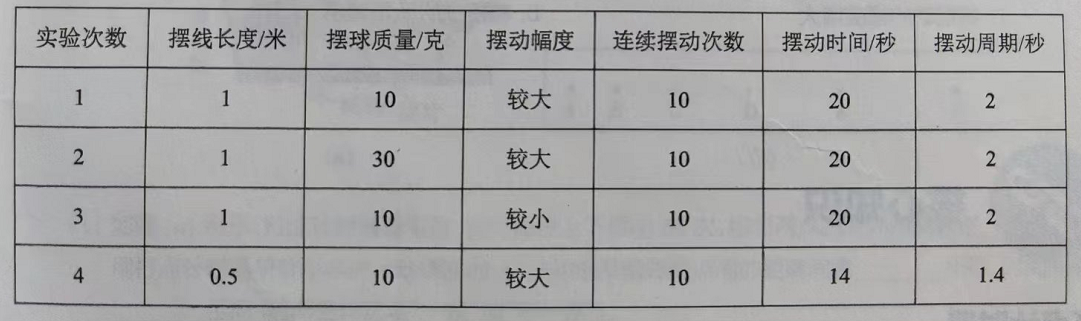
\includegraphics [scale=0.3,trim=0 0 0 0]{./image/fig_1_16.PNG}
    \caption{小明的试验记录} 
    \label{fig:fig_1_16}
\end{figure}
想一想,当摆钟走时过快时,我们可以怎样调整?


\end{groups}

\label{lastpage}
\end{document}